\section{Results}
\label{sec:results}

Determining the value for the threshold current requires careful adjustment of the unattenuated laser power. For the LED regime,
in which spontaneous emission dominates the light production, stable interference patterns cannot exist. This means that the
light on the IR viewing card appears diffuse and symmetrical. As soon as stimulated emission begins to dominate, the diode
operates in the LASER regime. The now coherent wave interacts with the texture of the card surface and creates a stable asymmetrical
image. The observed type of diffraction occurs due to the various bumps and grooves roughly matching the wavelength in size, resulting
in random granulation as predicted by Huygens principle. 

While lasing, the intensity also increases much more rapidly due to the strictly linear dependence on charge carrier flow.

\begin{figure}[H]
    \begin{subfigure}{0.48\textwidth}
        \centering
        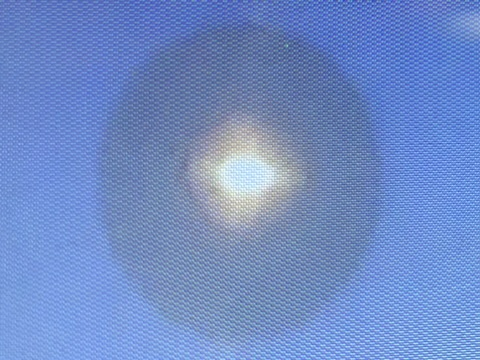
\includegraphics[width=\linewidth]{content/measurement/led.jpg}
        \caption{LED regime at $I = \qty{34.4}{\milli\ampere}$.}
        \label{fig:pattern_led}
    \end{subfigure}
    \hfill
    \begin{subfigure}{0.48\textwidth}
        \centering
        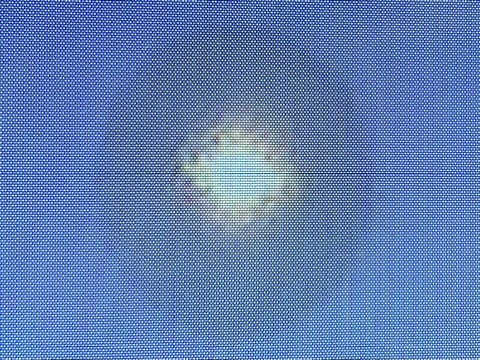
\includegraphics[width=\linewidth]{content/measurement/laser.jpg}
        \caption{LASER regime at $I = \qty{34.6}{\milli\ampere}$.}
        \label{fig:pattern_laser}
    \end{subfigure}
    \caption{Comparison of light pattern slightly below and above the chosen threshold current $I = \qty{34.5}{\milli\ampere}$.
             Note the diffuse reflection on the left versus the coarse granulation on the right. These distinct appearances
             are the results from random diffraction of incoherent or coherent waves respectively.}
    \label{fig:pattern}
\end{figure}

The described patterns can be viewed in Figure \ref{fig:pattern} for values slightly above and below the threshold. For the given
apparatus, visual examination yields $I = \qty{34.5}{\milli\ampere}$ as the minimum lasing current, though there is some ambiguity
as will be discussed later.

\begin{figure}[H]
    \centering
    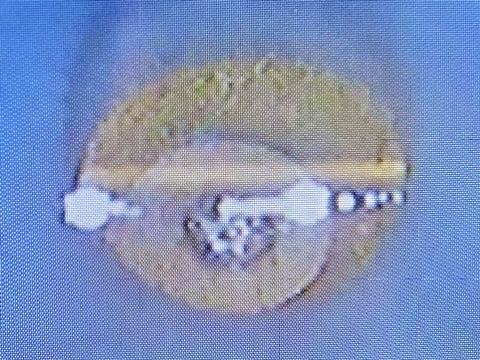
\includegraphics[width=0.48\linewidth]{content/measurement/fluorescence.jpg}
    \captionsetup{width=0.7\linewidth}
    \caption{Rubidium flourescence line along the laser beam as seen through the observation window in the vapor cell.}
    \label{fig:fluorescence}
\end{figure}

To find the approximate resonance of the rubidium fluorescence, laser current and grating angle are adjusted until a bright flashing
line along the path of the light beam manifests inside the vapor cell. To confirm this setting, Figure \ref{fig:fluorescence} displays
the observed excitation.

Following the previous steps, the hyperfine structure absorption spectrum of rubidium can be analysed. After iteratively tuning current
and DC offset values for the piezo stack, we arrive at Figure \ref{fig:ramp} without any mode hops.

\begin{figure}[H]
    \centering
    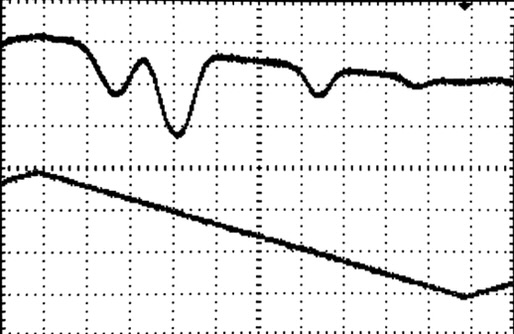
\includegraphics[width=0.72\linewidth]{content/measurement/ramp.jpg}
    \captionsetup{width=0.8\linewidth}
    \caption{Modulated signal without correction (top). Triggered ramp output for laser and piezo stack (bottom).
             As previously described, the expected linear proportionality between the two currents is clearly visible
             outside the absorption dips.}
    \label{fig:ramp}
\end{figure}

From this result, we finally obtain the corrected spectrum. Figure \ref{fig:spectrum} shows the signal shape after trying to
achieve a constant background outside of the peaks. The success of this technique is evaluated below.

\begin{figure}[H]
    \centering
    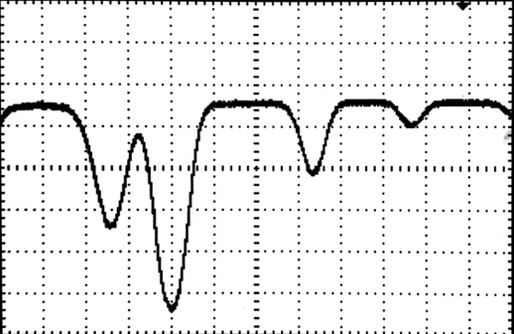
\includegraphics[width=0.72\linewidth]{content/measurement/spectrum.jpg}
    \captionsetup{width=0.8\linewidth}
    \caption{Spectrum after manual compensation via background subtraction for the scanning current contribution.}
    \label{fig:spectrum}
\end{figure}
